\documentclass{article}
\usepackage[T1]{fontenc}
\usepackage{lmodern}
\usepackage{graphicx}
\usepackage{amsmath,amssymb}
\usepackage[a4paper,margin=2cm]{geometry}
\usepackage[absolute,overlay]{textpos}
\setlength{\TPHorizModule}{1mm}
\setlength{\TPVertModule}{1mm}
\usepackage[indonesian]{babel}
\usepackage{hyperref}
\setlength{\emergencystretch}{2em}
% unit: Halaman 59

\begin{document}

% === Halaman 59 (llm) ===

\begin{itemize}
  \item Sedangkan di dalam cipher blok yang lain, permutasi tidak menggunakan P-box, tetapi melakukan pergeseran bit ke kiri atau ke kanan sejauh k bit.
  \item Pergeseran bersifat siklik, yaitu bit yang paling ujung muncul pada ujung yang lain
  \item Contoh pergeseran byte di dalam AES:
\end{itemize}

\vspace{10mm}

% deskripsi: Diagram proses ShiftRows pada AES yang menunjukkan transformasi state menjadi state' melalui pergeseran siklik pada setiap baris.
% bbox normalisasi: [0.1220, 0.5600, 0.8770, 0.9210]
\begin{textblock*}{158.55mm}(25.62mm,166.32mm)
\noindent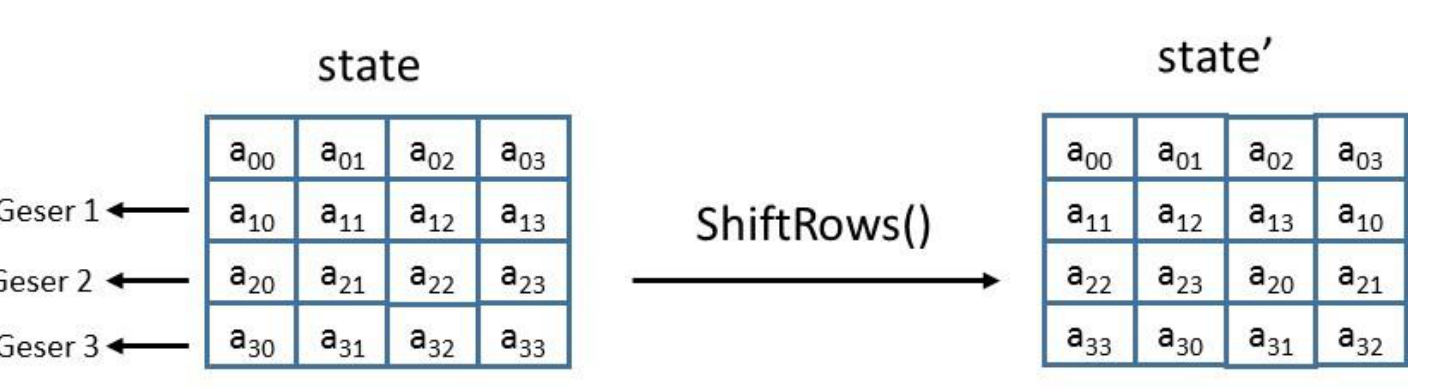
\includegraphics[width=158.55mm,height=107.22mm]{../../images/llm/page_059_img_01.png}%
\end{textblock*}

\end{document}
